\chapter{Related Works}

\begin{chaptersummary}
This chapter surveys prior work relevant to adaptive and enveloping grasping as well as tendon-driven laparoscopic end-effectors. It covers loop- and belt-based grippers, sensorized soft grippers, material and microstructure innovations, grasp planning algorithms, actuation technologies, sensing strategies, tip and rod architectures, soft and continuum approaches, and AI-assisted monitoring and control.

The review highlights recurring challenges, including cable coupling, material creep and stretch, frictional losses, and the trade-offs between flexibility, load capacity, and sensing complexity. It identifies open gaps that motivate this thesis: compact, tension-preserving cable routing; miniature sensing for closed-loop compensation; mechanism-level evaluations linking design choices to performance; and robust sensing and routing strategies for loop-based grippers, which Lasso Gripper seeks to explore as the main mechanism platform.
\end{chaptersummary}

\section{Advances in Actuation Technologies for Multi-DOF End-Effectors in Laparoscopic Instruments}

Minimally Invasive Surgery (MIS) shifted instrument design toward restoring distal dexterity within severe access constraints. Cable-driven actuation is widely used because it enables multi-degree-of-freedom tips with low distal mass, but it brings challenges such as cable coupling, material creep, and reduced control fidelity. This section summarizes actuation alternatives, sensing strategies for tension and pose estimation, and tip/shaft design patterns that motivate the tendon-driven choices explored in this thesis.

To address the limited dexterity at the instrument tip, a prominent solution involves using cables as a medium to transmit power from the handpiece to the end-effector, thereby enabling additional DOFs, such as roll or yaw rotations. First introduced in the late 1990s, Intuitive Surgical's da Vinci system exemplifies this approach, employing a cable-driven mechanism to control its articulated tips. The primary advantage of such a system is that cables can transmit power over a distance with a lower weight penalty compared to rigid linkages or gear trains\cite{brodie_future_2018}. However, this benefit is accompanied by inherent challenges. In the initial design of the da Vinci system, cable coupling, where the movement of one cable inadvertently affects another, was a significant issue that could not be overlooked, often leading to kinematic inaccuracies and reduced control fidelity. Therefore, various approaches have been studied to address these problems.

\subsection{Replacements of Driven Motors}
\begin{figure}[htbp]
\centering
\begin{subfigure}[t]{0.48\textwidth}
\centering
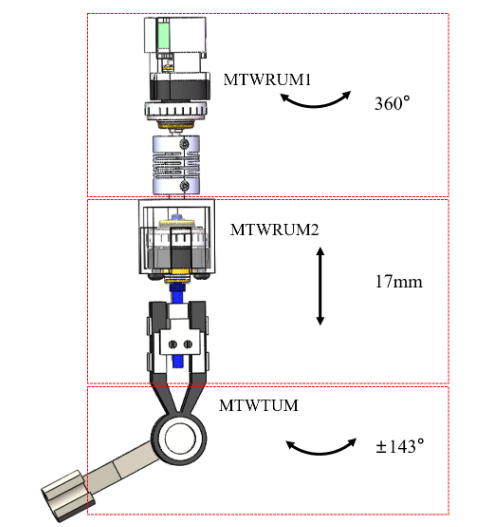
\includegraphics[width=\linewidth]{Figures/magnetic.png}
\caption{Design and illustration of ultrasonic motors\cite{li_design_2022}.}
\label{fig31a}
\end{subfigure}
\hfill
\begin{subfigure}[t]{0.48\textwidth}
\centering
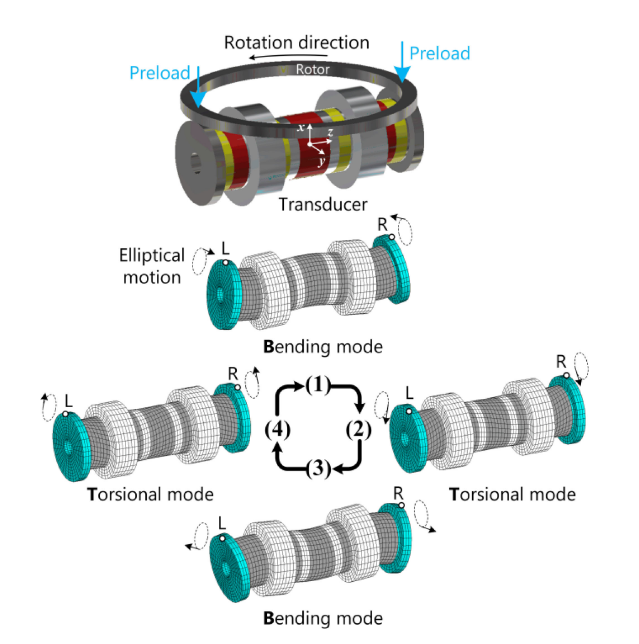
\includegraphics[width=\linewidth]{Figures/bending torsion.png}
\caption{Bending and torsion layouts of the transducer\cite{wu_rotary_2021}.}
\label{fig31b}
\end{subfigure}

\vspace{0.5em}

\begin{subfigure}[t]{0.48\textwidth}
\centering
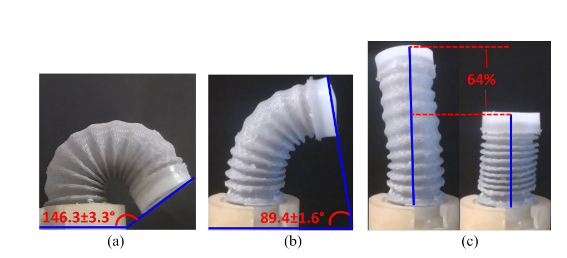
\includegraphics[width=\linewidth]{Figures/soft modular.png}
\caption{Flexible fluidic actuators with granular jamming for variable stiffness\cite{ranzani_soft_2016}.}
\label{fig31c}
\end{subfigure}
\hfill
\begin{subfigure}[t]{0.48\textwidth}
\centering
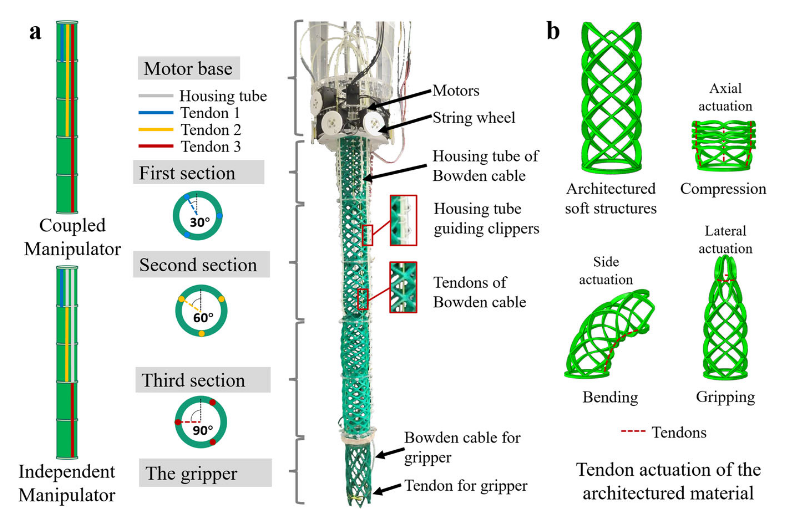
\includegraphics[width=\linewidth]{Figures/trimmed.png}
\caption{The tendon-driven manipulator design with trimmed helicoids\cite{guan_trimmed_2023}.}
\label{fig31d}
\end{subfigure}

\caption{Selected actuation and compliant tip technologies from recent MIS research. (a) ultrasonic motors; (b) bending and torsion transducer layouts; (c) flexible fluidic actuators with granular jamming for variable stiffness; (d) tendon-driven trimmed helicoid manipulator.}
\label{fig31}
\end{figure}

To address the challenges of control fidelity loss and restricted tip articulation in minimally invasive surgical instruments, various driving mechanisms have been extensively investigated. One prominent approach involves the implementation of ultrasonic motors as alternatives to conventional electromagnetic actuators. As illustrated in Fig. \ref{fig31a}, experimental validation has confirmed that the maximum output torque reaches $1.2\,\mathrm{mN\,m}$ for the rotary configuration and $1.4\,\mathrm{mN\,m}$ for the tilting mechanism. These torque values adequately satisfy the operational requirements of magnetically anchored laparoscopes while offering superior positional precision. Crucially, performance evaluations of the prototype system have substantiated both the feasibility and effectiveness of integrating these ultrasonic motors into laparoscopic applications\cite{kiong_tan_precision_2015}. This approach presents a novel and practical alternative for achieving enhanced visual platform maneuverability in single-port surgery, addressing fundamental limitations in conventional cable-driven systems through improved torque transmission and positioning accuracy.

Some studies focus on matching the power density and peak torque output of this proposed driving method to those of electromagnetic actuators. By applying a rod-shaped transducer in torsional and bending modes, the rotor is driven in its orthogonal direction with external excitations at specific frequencies. By adjusting the excitation frequencies, the maximum torque recorded in the experiments reached $10.1\,\mathrm{N\,m}$, and the output power reached $38.1\,\mathrm{W}$\cite{wu_rotary_2021}.

\subsection{Additional Sensors}

A fundamental limitation in the original cable-driven system involves the progressive uncertainty of cable length resulting from material creep during prolonged operation. This phenomenon introduces cumulative positioning errors between the input and output ends, significantly compromising control fidelity\cite{liang_novel_2017}. To mitigate this inherent uncertainty, the integration of supplemental sensing modalities has been implemented. These sensors enable real-time monitoring of either cable tension, end-effector pose, or both, facilitating a closed-loop control architecture that dynamically compensates for length variations and restores positional accuracy.



Accurate measurement of cable tension during surgical procedures represents a critical safety requirement in cable-driven robotic systems. In traditional laparoscopic surgery, surgeons rely on haptic feedback transmitted through rigid instruments to assess tissue interaction forces. However, in motor-driven systems where actuation forces are generated remotely, this crucial tactile information becomes significantly attenuated. This sensory disconnect necessitates extensive training for surgeons to develop appropriate motor control through the handheld interface, as demonstrated in studies on force sensing in robotic surgery \cite{trejos_force_2010}.

Force sensing has emerged as a promising solution to restore this lost feedback. The most straightforward approach involves embedding force sensors, such as Fiber Bragg Gratings (FBGs), directly into the surgical instrument. As explored in research on mechatronic design of force sensors\cite{zemiti_mechatronic_2007}, this method enables direct measurement of interaction forces at the end-effector. However, this integration often results in structural redundancy and increased instrument diameter, creating bulky designs that may compromise surgical access and maneuverability in confined operative fields.

To address these limitations, recent research has focused on miniaturized sensing strategies. One innovative approach involves embedding FBGs within precisely machined grooves on inclined cantilevers within the instrument structure\cite{xue_design_2018}. This design exploits the strain measurement capabilities of FBGs to detect minute deformations in the cantilevers caused by cable tension variations. The inclined configuration amplifies these deformations, enabling high-sensitivity force measurement while maintaining a compact form factor compatible with the dimensional constraints of minimally invasive instruments.

\subsection{Novel Structures of the Tip and Rod Design }

In conventional master-slave robotic systems, such as the da Vinci Surgical System and similar handheld robotic instruments, the end-effector typically provides 4 to 5 DOFs. This configuration is designed to replicate the articulation capabilities of the human wrist and fingers, enabling complex maneuvers like pitching, yawing, rolling, and grasping. However, a significant design limitation persists: these multiple DOFs are concentrated exclusively at the distal tip, while the connecting shaft or linkage primarily functions as a passive rotary base.

This recognition of ergonomic limitations in conventional articulated instruments has stimulated significant research into alternative tip architectures in recent years. With advances in the modeling and control of continuum robots, their design principles have been increasingly translated into the medical domain. Unlike traditional tip designs composed of multiple rigid links connected by discrete joints, continuum robots offer a validated scheme for implementing soft or continuously flexible connections, both between the tip and the instrument shaft, and among individual subcomponents of the tip itself. This paradigm shift enables a more distributed deformation along the instrument's length, effectively increasing the overall dexterity without concentrating all articulation at a single point. The resulting designs, often drawing inspiration from biological structures like tentacles or snakes, promise to mitigate surgeon fatigue by decoupling the end-effector's pose from the precise position of the surgeon's hand, thereby offering a more intuitive and ergonomic manipulation platform for complex surgical tasks.
Building upon the foundational research in continuum robotics, recent studies have explored innovative structural designs to enhance surgical instrument dexterity and safety. Ranzani et al. (2016) demonstrated a significant advancement by integrating flexible fluidic actuators within a silicone matrix containing multiple pneumatic chambers. This design enabled multidirectional bending and elongation capabilities. The proposed manipulator employed a modular architecture, utilizing granular jamming techniques to achieve dynamic stiffness variation and diverse movement profiles, as illustrated in Fig.~\ref{fig31c}.
Further extending this paradigm, researchers have investigated the transition from rigid linkages to compliant structures to substantially improve operational flexibility. One notable approach involves manipulating the trimmed angle of a helicoid structure to create a variable-stiffness robotic arm\cite{guan_trimmed_2023}. When coupled with a cable-driven actuation system, this design achieves an expanded workspace while significantly minimizing the risk of iatrogenic tissue damage during surgical procedures, as shown in Fig.~\ref{fig31d}. These developments in soft robotics and variable-stiffness mechanisms represent promising directions for next-generation surgical instruments that balance precision with patient safety.

\subsection{AI-Assisted Monitoring and Control}
As analyzed in previous sections, contemporary research in medical instrumentation predominantly advances along three interconnected fronts: innovative tip design, integrated sensory feedback systems, and intelligent control algorithms. The rapid evolution of Deep Learning and Reinforcement Learning methodologies has now catalyzed a fourth research direction: the integration of data-driven approaches into clinical practice.

A particularly promising development lies in repurposing the existing endoscopic camera, initially intended solely for surgical visualization, as an external verification system for instrument navigation. Specifically, Kong et al. (2023) demonstrated that through a specially designed architecture, both the visual stream from the camera and kinematic data from the actuation motors can be fused to estimate the positional discrepancy between commanded and actual end-effector positions following movement execution\cite{kong_automatic_2023}. This estimated deviation is subsequently converted into compensation signals that drive automatic self-correction maneuvers, effectively creating a vision-enhanced closed-loop control system that continuously calibrates the instrument without requiring additional hardware beyond the standard surgical setup.

This methodology represents a significant paradigm shift from traditional model-dependent control strategies, leveraging the wealth of available surgical video data to address inherent system limitations such as cable stretch, hysteresis, and kinematic modeling inaccuracies. The approach demonstrates how computer vision and deep learning techniques can transform existing surgical infrastructure into a self-calibrating system, potentially enhancing both positioning accuracy and long-term reliability in cable-driven surgical instruments.

\subsection{Synthesis of Design Gaps for Handheld Tendon-Driven Instruments}

The reviewed literature shows that no single design direction fully resolves the practical requirements of a handheld multi-DOF surgical instrument. Distal motors and ultrasonic actuators can improve local responsiveness, but they tend to increase distal complexity and may create packaging or thermal-management concerns. Cable-driven and tendon-driven architectures relocate actuation proximally and therefore reduce distal mass, but introduce nonlinear transmission effects such as coupling, backlash, friction, and hysteresis. Continuum and soft structures improve access and safety, yet their compliance can make precise tip positioning and high-load manipulation more difficult without additional sensing or compensation.

These trade-offs motivate the design strategy adopted in this thesis. Rather than treating actuation, sensing, routing, and control as separate subproblems, the proposed handheld instrument is organized around explicit tension management. The mechanical layout preserves proximal actuation, paired cable routing, and quick-swap modularity; the input stage separates user-intent sensing from distal actuation; and the control implementation uses low-level servo feedback to constrain cable motion. Table~\ref{tab:surgical_lit_synthesis} summarizes the main design implications extracted from the related work and maps them to the design decisions used later in the thesis.

\begin{table}[htbp]
    \centering
    \caption{Synthesis of surgical-instrument literature and implications for this thesis}
    \label{tab:surgical_lit_synthesis}
    \begin{tabular}{p{0.23\linewidth} p{0.25\linewidth} p{0.24\linewidth} p{0.18\linewidth}}
        \toprule
        Research direction & Main advantage & Remaining limitation & Thesis response \\
        \midrule
        Distal or miniature actuation & Direct local actuation and high responsiveness & Added distal mass, packaging difficulty, and possible heat or wiring burden & Keep heavier actuation proximal and transmit motion through cables \\
        Cable/tendon transmission & Low distal inertia and compact multi-DOF motion & Coupling, backlash, friction, cable stretch, and hysteresis & Use paired winding, guided routing, and feedback-supported tension management \\
        Embedded force or shape sensing & Improved safety and closed-loop compensation & Increased structural complexity and integration burden & Use compact input sensing and servo-state feedback in the current prototype \\
        Soft and continuum mechanisms & Compliance, safety, and large bending range & Reduced stiffness and harder high-precision control & Retain rigid load-bearing tip while using cable compliance for safer interaction \\
        Vision and learning-based compensation & Potential correction of unmodeled errors & Requires training data, validation, and robust perception & Reserved as a future calibration and adaptive-control pathway \\
        \bottomrule
    \end{tabular}
\end{table}

This synthesis also clarifies the relationship between the surgical instrument and Lasso Gripper. Both systems rely on flexible tensile elements to transmit motion and regulate interaction forces, but they emphasize different operating regimes and play different roles in the thesis. Lasso Gripper is the primary mechanism contribution and uses a free loop to maximize capture tolerance in open manipulation. The surgical instrument is a complementary application case that constrains the cable path through guide tubes, pulleys, and reels to maximize repeatability in a compact handheld device. The literature review therefore motivates a common mechanism question for the remainder of the thesis: how can flexible tensile transmission be designed so that its compliance is useful rather than a source of uncontrolled error?
